
%----------------------------------------------------------------------------------------
%	PACKAGES AND OTHER DOCUMENT CONFIGURATIONS
%----------------------------------------------------------------------------------------

\documentclass[twocolumn]{article}

\usepackage[sc]{mathpazo} % Use the Palatino font
\usepackage[T1]{fontenc} % Use 8-bit encoding that has 256 glyphs
\linespread{1.05} % Line spacing - Palatino needs more space between lines
\usepackage{microtype} % Slightly tweak font spacing for aesthetics

\usepackage{blindtext} % Package to generate dummy text throughout this template

\usepackage{amssymb}

\usepackage[margin=0.6in]{geometry}

\usepackage{hyperref} % For hyperlinks in the PDF
\hypersetup{
  colorlinks   = true, %C olours links instead of ugly boxes
  urlcolor     = blue, % Colour for external hyperlinks
  linkcolor    = blue, % Colour of internal links
  citecolor   = blue % Colour of citations
}

\usepackage{flushend}	% Balance columns on last page 

\usepackage{graphicx}

\usepackage[hang, small,labelfont=bf,up,textfont=normal,up]{caption} % Custom captions under/above floats in tables or figures

\usepackage{paralist} % Used for the compactitem environment which makes bullet points with less space between them

\usepackage{abstract} % Allows abstract customization
\renewcommand{\abstractnamefont}{\large\bfseries} % Set the "Abstract" text to bold
\renewcommand{\abstracttextfont}{\normalfont\normalsize} % Set the abstract text properties

\usepackage{fixltx2e} % Subscript and superscript in text mode (\textsuperscript{} and \textsubscript{})

\usepackage{acronym} % Acronyms

\usepackage{titlesec} % Allows customization of titles
\titleformat{\section}[block]{\large\scshape\centering{\Roman{section}.}}{}{1em}{} % Change the look of the section titles 
\titleformat*{\subsection}{\normalsize\bfseries} % Set subsection style to normalsize and bold


%----------------------------------------------------------------------------------------
%	TITLE SECTION
%----------------------------------------------------------------------------------------

\title{\vspace{-10mm}\fontsize{20pt}{10pt}\selectfont\textbf{Dimensionality reduction for \acs{emg} prediction of upper-limb activity from \acs{lfp} recordings in primates\\} % Article title
\vspace{1cm}
\large \textbf{Research proposal for MSc by Research Thesis}\\
DTC Neuroinformatics and Computational Neuroscience\\
\vspace{0.5cm}
}

\author{
%\textbf{Agamemnon Krasoulis}\\
\textbf{Proposed by}\\
Agamemnon Krasoulis\\
\href{mailto:a.krasoulis@sms.ed.ac.uk}{\nolinkurl{a.krasoulis@sms.ed.ac.uk}}
\and
\textbf{Principal supervisor}\\
Dr. Kianoush Nazarpour\\
\href{mailto:kianoush.nazarpour@touchbionics.com}{\nolinkurl{kianoush.nazarpour@touchbionics.com}}
\and
\textbf{Second supervisor}\\
Prof. Sethu Vijayakumar\\
\href{mailto:sethu.vijayakumar@ed.ac.uk}{\nolinkurl{sethu.vijayakumar@ed.ac.uk}}
}


%\renewcommand\Authands{ and }
%----------------------------------------------------------------------------------------
%  ACRONYMS
%----------------------------------------------------------------------------------------

\acrodef{eeg}[EEG]{electroencephalogram}
\acrodef{emg}[EMG]{electromyogram}
\acrodef{anova}[ANOVA]{analysis of variance}
\acrodef{lfp}[LFP]{local field potential}
\acrodef{mua}[MUA]{multi-unit activity}
\acrodef{pca}[PCA]{principal component analysis}
\acrodef{m1}[M1]{primary motor cortex}
\acrodef{bmi}[BMI]{brain-machine interface}
\acrodef{fes}[FES]{functional electrical stimulation}
\acrodef{sci}[SCI]{spinal cord injury}
\acrodef{nmp}[NMP]{neuro-motor prosthesis}
\acrodef{efp}[EFP]{epidural field potential}
\acrodef{lmp}[LMP]{local motor potential}
\acrodef{r2}[$R^2$]{coefficient of determination}
\acrodef{vaf}[VAF]{variance accounted for}
\acrodef{mlp}[MLP]{multilayer perceptron}
\acrodef{cm}[CM]{corticomotoneuronal}
\acrodef{vkf}[Velocity-KF]{velocity Kalman filter}
\acrodef{rekf}[ReFIT-KF]{recalibrated feedback intention-trained Kalman filter}
\acrodef{Bmi}[BMI]{Brain-machine interface}
\acrodef{ecog}[ECoG]{electrocorticography}
\acrodef{pmv}[PMv]{ventral premotor cortex}
\acrodef{bic}[Bi]{biceps}
\acrodef{ecr}[ECR]{extensor carpi radialis}
\acrodef{fcu}[FCU]{flexor carpi ulnaris}
\acrodef{ecu}[ECU]{extensor carpi ulnaris}
\acrodef{fcr}[FCR]{flexor carpi radialis}
\acrodef{tri}[Tri]{triceps}
\acrodef{fds}[FDS]{flexor digitorum superficialis}
\acrodef{fdp}[FDP]{flexor digitorum profundus}
\acrodef{1di}[1DI]{first dorsal interosseous}
\acrodef{fft}[FFT]{fast fourier transform}
\acrodef{cc}[CC]{coefficient of correlation}
\acrodef{nrmse}[nRMSE]{normalised root-mean square error}
\acrodef{slir}[SLiR]{sparse linear regression}
\acrodef{vb}[VB]{variational bayes}
\acrodef{vbls}[VBLS]{variational Bayesian least squares}
\acrodef{nrmse}[nRMSE]{normalised root-mean-square error}
\acrodef{lasso}[LASSO]{least absolute shrinkage and selection operator}
\acrodef{ard}[ARD]{automatic relevance detection }
%----------------------------------------------------------------------------------------

%----------------------------------------------------------------------------------------
%	MACROS
%----------------------------------------------------------------------------------------

\newcommand{\slfrac}[2]{\left.#1\middle/#2\right.} % Size properly the slash symbol in equations
%----------------------------------------------------------------------------------------

%----------------------------------------------------------------------------------------
% 	DOCUMENT
%----------------------------------------------------------------------------------------

\begin{document}
\twocolumn[
  \begin{@twocolumnfalse}
  \date{}
\vspace{5mm}
\maketitle % Insert title


%----------------------------------------------------------------------------------------
%	ABSTRACT
%----------------------------------------------------------------------------------------

\begin{abstract}

\noindent Neural prosthetic systems aim to assist patients suffering from sensory, motor and other disabilities by translating neural brain activity into control signals for assistive devices, such as computers and robotics prostheses, or by restoring muscle contraction through \ac{fes}. In a neuro-motor prosthetic device, the prediction of intended muscle electrical activity is required for effective \ac{fes}. It has been already known that upper-limb \ac{emg} signals in primates can be accurately predicted by decoding the spike activity of single and multi-units in the \ac{m1}. Recent work now suggests that \ac{emg} signals can also be decoded by \ac{lfp} recordings in \ac{m1}. In such decoding schemes, the number of input variables is usually very large and no systematic way of performing effective variable selection has yet been suggested. The proposed research project will investigate the potential benefit of using dimensionality reduction and sparse variable selection techniques for predicting upper-limb \ac{emg} activity, based on recorded \ac{lfp} signals in the \ac{m1} and \ac{pmv} of primates. The study will use already existing datasets coming from two freely-behaving animals. Prediction accuracy with different techniques will be evaluated, and compared to results reported in the literature. 
\end{abstract}
\vspace{7mm}
   \end{@twocolumnfalse}
]

\acresetall % Reset all acronyms

%----------------------------------------------------------------------------------------
%	ARTICLE CONTENTS
%----------------------------------------------------------------------------------------
\section{Introduction}

Electrical activity in the \ac{m1} has been found to correlate with both kinematic (e.g. position and velocity) \cite{Georgopoulos1982}, and kinetic (e.g. force) \cite{Evarts1968} aspects of movement. These findings have led to the inspiration and development of \acp{bmi}, which by recording activity from motor cortical areas allow users to move a computer cursor \cite{Paninski2002, Carmena2003, Hochberg2006} or a robotic limb \cite{Velliste2008}. In some cases, muscle contraction of temporarily paralysed animals \cite{Ethier2012} or patients with tetraplegia \cite{Peckham2001} has been achieved through \ac{fes}, and found to be effective in allowing subjects to regain control of basic hand movements. Worldwide, thousands of people suffering from \ac{sci}, brainstem strokes or other disorders, would potentially benefit from neuro-motor prosthetic devices \cite{Hochberg2006}.

\par The operation of a \ac{nmp} can be divided into four major components; signal acquisition, signal/information processing, neural decoding and control signal generation for artificial limb movement \cite{Linderman2008}. Most studies \cite{Hochberg2006, Hochberg2012, Ethier2012, Nazarpour2012, Pohlmeyer2007}, have used multielectrode arrays to record single and multi-unit spike activity, which was then used as the source signal for decoding intended hand movements. Motion-related spike activity has been found to be present  in the \ac{m1} even after three years of \ac{sci} \cite{Hochberg2006}. For effective \ac{fes}, an accurate mechanism for prediction of \ac{emg} signals is needed, and many methods spanning from linear \cite{Carmena2003}, Wiener cascade models \cite{Pohlmeyer2007} and Kalman filters \cite{Wu2006, Wu2009, Nazarpour2012} have been proposed in the literature.

\par Recently, it has been found \cite{Flint2012,Flint2012a} that \ac{lfp} recordings can also be used to decode upper limb activity in primates. In these studies it was shown that position and velocity decoding, as well as \ac{emg} prediction, can be achieved from \ac{lfp} signals with accuracy nearly as high as with spike signals. The advantages of using \ac{lfp} signals instead of spike activity signals, as source signals for \acp{bmi} are numerous; firstly, the bandwidth is significantly lower (sampling rate at 1 kHz instead of 30 kHz for spike signals), which translates into lower power requirements for the processor of the \ac{bmi}. Secondly, single-unit activity is difficult to record for a long time after the implantation. Another study has also shown that \ac{emg} prediction can be achieved by using \ac{ecog} signals \cite{Shin2012}, which are measured with electrodes placed on the surface of the brain, thus constituting a less invasive candidate for \acp{bmi} source signals.

\section{Motivation}

The proposed study will focus on upper-limb \ac{emg} activity prediction in primates, by using \ac{lfp} signals recorded in the animals' \ac{m1} and \ac{pmv}. 

\par The first novelty of the study is that recordings come from freely-behaving animals, in comparison with most studies in the literature, which investigate \ac{emg} prediction during center-out reaching tasks. Hence, we will  seek to investigate whether decoding is also possible during free behaviour, or whether it is limited only to repetitive tasks. 

\par The second novelty will consist in applying dimensionality reduction techniques for predicting \ac{emg} signals. \ac{lfp} signals are usually highly-correlated, and it has also been shown that some \ac{lfp} frequency bands are more correlated to \ac{emg} activity than others \cite{Flint2012, Rickert2005}. Furthermore, decoding \ac{emg} activity from \ac{lfp} recordings usually involves extracting a very large number of features. In order to deal with this curse of dimensionality, two different techniques have been proposed in the literature. In \cite{Flint2012}, the 150 features which were most strongly correlated with the \ac{emg} signals were selected, by computing the absolute values of the Pearson-r correlation coefficients. In \cite{Shin2012}, where \ac{emg} activity was predicted by using \ac{ecog} signals, a \ac{slir} algorithm based on a \ac{vb} method \cite{Sato2001} was used. Other methods, such as neuron dropping \cite{Pohlmeyer2007}, and a \ac{vbls} approach \cite{Ting2010} have been used in paradigms where \ac{emg} activity is predicted by using spike trains (rate coding) from neurons in \ac{m1}.

\par Our objective will be to use dimensionality reduction techniques to perform effective sparse variable selection, and subsequently test \ac{emg} prediction accuracy based on the selected variables.

\section{Datasets}

The available datasets come from recordings from two freely-behaving animals. During the recordings, the animals were offered food in a peg-board that had holes of 1-cm diameter. The behavioural task comprised reaching the board, picking up the food and putting it into the animals' mouth. The duration of the two recording sessions is 15.26 and 5.79 min, respectively. The datasets comprise recordings from:
\begin{itemize}
\item Spike activity of 56 single units in the \ac{m1} (44/56) and the \ac{pmv} (12/56)
\item 56 \ac{lfp} channels in the same areas
\item 9 \ac{emg} signals from the following muscles (see Fig. \ref{fig:muscles}): \ac{ecr}, \ac{fcu}, \ac{bic}, \ac{ecu}, \ac{fcr}, \ac{tri}, \ac{1di}, \ac{fds}, \ac{fdp}
\end{itemize}

\begin{figure}[ht]
\centering
	\includegraphics[width=0.48\textwidth]{muscles.pdf}
\caption{Schematic of recorded limb muscle locations. Both medial (\textbf{A}) and lateral (\textbf{B}) views are shown. Adapted from \cite{Flint2012}.}
\label{fig:muscles}
\end{figure}

Fig. \ref{fig:raw_data} shows an example of the raw data containing the spike activity of 10 units in \ac{m1}, two \ac{lfp} channels and two \ac{emg} signals. The duration of the shown excerpt is 6 s.
 
\begin{figure}[ht]
\centering
	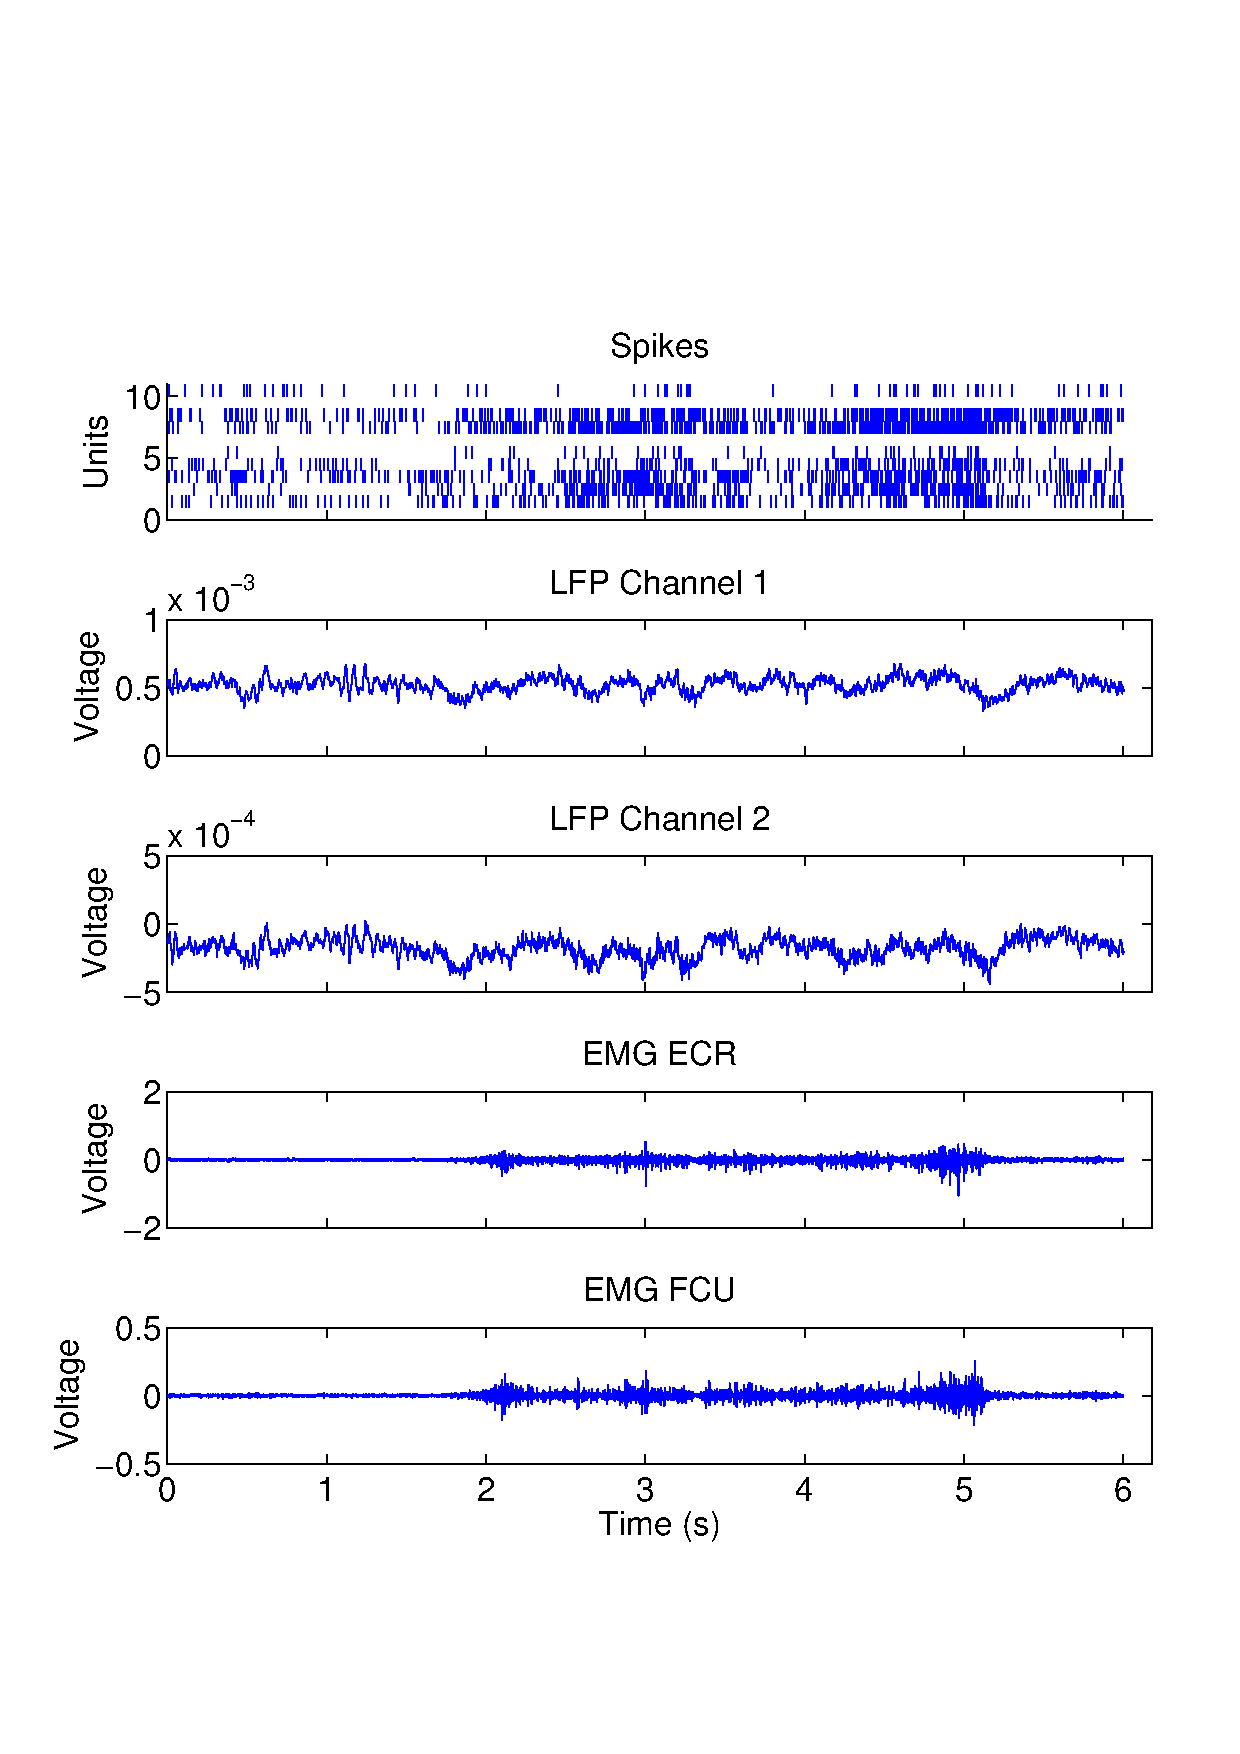
\includegraphics[width=0.48\textwidth]{raw_data.pdf}
\caption{Raw data. The spike activity of 10 single-units is shown, along with two \ac{lfp} channels and the \ac{emg} signals from \ac{ecr} and \ac{fcu} muscles. }
\label{fig:raw_data}
\end{figure}

\section{Methods}
\subsection{Signal processing}
For the \acp{emg}, the signals envelopes will be extracted and used for the decoding process. Thus, the signals will be high-pass filtered at 50 Hz, full-wave rectified, low-pass filtered at 5 Hz and finally downsampled to 20 Hz. All filters will be applied forward and backward in time, to avoid phase delays \cite{Flint2012}.

For each \ac{lfp} signal, six spectral features will be used: the \ac{lmp}, which is a sliding window average of the raw \ac{lfp}, and the power in five frequency bands (0-4, 7-20, 70-115, 130-200, and 200-300 Hz). The power in each band will be computed by applying a Hanning window and the \ac{fft} . All features will be computed in 256-point windows, with 206-point overlaps. 

\subsection{Model fitting}
For fitting \ac{emg} envelopes to \ac{lfp} signals, we will explore the potential benefit of using a variety of methods, which include but are not limited to:
\begin{itemize}
\item the \ac{lasso} technique \cite{Tibshirani1996} is a method for linear regression which results in sparse interpretable models, by shrinking certain regression coefficients exactly to zero. The shrinkage effect of the method arises naturally from using a penalty for the L\textsubscript{1} norm of the coefficient vector. One drawback of the algorithm is that the regularization parameter needs to be set manually.
\item the elastic net \cite{Zou2005} is an extension of the \ac{lasso} which, by introducing an additional penalty on the L\textsuperscript{2} norm, encourages a group effect of the variables, in a way that correlated variables tend to be in or out of the model together.
\item the online \ac{vb} method \cite{Sato2001} uses a Bayesian approach to perform model selection. The free energy is defined for a trial distribution, and it can be shown that its maximisation gives the true posterior distribution.
\item the \ac{vbls} is also a Bayesian approach to linear regression, which by performing \ac{ard} of the input variables, excludes the ones that are irrelevant to the data, resulting thus in sparse representations.
\end{itemize}
Tools that will be potentially used include the SpaSM (Sparse statistical modelling toolbox for MATLAB\textsuperscript{\textregistered}) \cite{Sjostrand2012} and the VBSR (Variational Bayesian Sparse Regression) \cite{Sato2009} and Variational Bayesian Least Squares  \cite{vblstool} toolboxes for MATLAB\textsuperscript{\textregistered}.
\section{Evaluation of performance}

The \ac{emg} prediction accuracy (similarity between actual and predicted \ac{emg} activity) can be evaluated by using various measures, such as:
\begin{itemize}
\item the proportion of the \ac{vaf}, which is a similar measure to the \ac{r2}, and is defined as follows:
\begin{equation}
VAF = 1 - \frac{\sum\limits_{j=1}^{M}\left(p_j-\hat{p_j}\right)^2}{\sum\limits_{j=1}^M\left(p_j-\bar{p}\right)^2}
\end{equation}


\item the \ac{cc}, given by:
\begin{equation}
CC = \frac{\sum\limits_{j=1}^{M}\left(p_j-\bar{p}\right)\left(\hat{p_j}-\bar{\hat{p}}\right)}{\sqrt{\sum\limits_{j=1}^{M}\left(p_j-\bar{p}\right)^2} 
\sqrt{\sum\limits_{j=1}^{M}\left(\hat{p_j}-\bar{\hat{p}}\right)}}
\end{equation}

\item the \ac{nrmse}, defined as:
\begin{equation}
nRMSE = \slfrac {\sqrt{\frac{\sum\limits_{j=1}^M \left(p_j - \hat{p_j} \right) ^2}{n}}}  {\left(p_{max}-p_{min} \right)}
\end{equation}
\end{itemize}
where $M$ is the number of samples of a dataset, $p_j$ and $\hat{p_j}$ are the actual and predicted values of the \ac{emg} signal for the j\textsuperscript{th} sample, $\bar{p}$ and $\bar{\hat{p}}$ denote the mean values  of the actual and predicted signals within the dataset, and $p_{max}$ and $p_{min}$ are the maximum and minimum values, respectively, of the actual signal.

\par Our results will be compared to \cite{Flint2012}, where a decoding technique based on a Wiener cascade model was used, and variable selection was performed by choosing the 150 features which were more strongly correlated with the \ac{emg} signals. 

\begin{table*}
\begin{center}
    \begin{tabular}{|l|l|}
        \hline
        May 2013    & Literature review \\
        				& Background reading on \ac{emg} prediction from \ac{lfp} recordings                     \\
        ~           & Background reading on dimensionality reduction and sparse variable selection techniques \\ 
        ~           & Earn familiarity with available datasets                                                \\  \hline
        June 2013   & Replication of results in \cite{Flint2012} 
        \\ 
        ~           & \ac{emg} prediction with LASSO                                                          \\ 
        ~           & \ac{emg} prediction with elastic-net                                                    \\  \hline
        July 2013   & \ac{emg} prediction with online \ac{vb}                                                      \\ 
        ~           & \ac{emg} prediction with \ac{vbls}                                                \\ 
        ~           & Analysis of results and comparison to \cite{Flint2012}                                  \\  \hline
        August 2013 & Thesis write-up                                                                         \\
        \hline
    \end{tabular}
    \end{center}
\hfill{}
\caption{Timeline of the proposed research project}
\label{tb:timeline}
\end{table*}

\begin{table*}
\begin{center}


 \begin{tabular}{|l|c|c|}
    \hline \
    ~                                          & \textbf{Quantity} & \textbf{Price (\textsterling)}       \\ \hline %\hline
    16-25 Railcard                             & 1        & 28              \\ \hline
    Return tickets from Edinburgh to Livingston & 13       & 13 X 5.5 = 71.5 \\ \hline %\hline
    \textbf{Total}                             & ~        & 99.5            \\ \hline
    \end{tabular}
    \end{center}
\caption{Budget of the proposed research project}
\label{tb:budget}
\end{table*}

\section{Roles of supervisors}

Each of the two supervisors has their own field of expertise. Dr. Kianoush Nazarpour has a long experience in signal processing research for \acp{bmi} for motor rehabilitation, and currently holds a position of senior algorithm engineer at Touch Bionics, Livingston, UK. He also holds a position of visiting researcher at the Motor Control Group, Institute of Neuroscience, University of Newcastle. He will serve as the principal supervisor of the project and will provide guidance, as well as the datasets used for the analyses. Prof. Sethu Vijayakumar holds the position of Professor of Robotics and Director of the Institute for Perception, Action and Behavior (IPAB) at the School of Informatics, University of Edinburgh, UK. He will be serving as the internal supervisor. The student is planning to have weekly meetings with the principal supervisor in Livingston, and with the internal supervisor in Edinburgh.

\section{Timeline}
A detailed timeline of the proposed research project is given in Table \ref{tb:timeline}.

\section{Budget}
The student will need to travel weekly to Livingston to hold meetings with the principal supervisor. The travel expenses are not expected to exceed \textsterling 100 in total, and a detailed description is given in Table \ref{tb:budget}.

%\newpage
\begin{center}
\line(1,0){125} % Line before references
\end{center}
\addtocounter{section}{1} % Increase counter for references

\renewcommand{\section}[2]{} % Hide references title

\bibliography{Bibliography}
\bibliographystyle{ieeetr}
\end{document}
